\documentclass[11pt]{article}
\usepackage[a4paper,margin=2.4cm]{geometry}
\usepackage[T1]{fontenc}
\usepackage{mathptmx}
\usepackage[scaled=0.9]{helvet}
\usepackage{courier}


\usepackage{amsmath,amssymb}
\usepackage{booktabs}
\usepackage{multirow}
\usepackage{xcolor}
\usepackage{tikz}
\usetikzlibrary{arrows.meta,positioning,fit,calc,decorations.pathreplacing}
\usepackage{caption}
\usepackage{enumitem}
\usepackage[colorlinks=true,linkcolor=blue!50!black,citecolor=blue!50!black,urlcolor=blue!50!black]{hyperref}
\usepackage{tcolorbox}
\usepackage{listings}
\lstset{basicstyle=\ttfamily\scriptsize,breaklines=true,columns=fullflexible,frame=single,framerule=0.3pt}

\newcommand{\pend}[1]{\textcolor{orange!80!black}{[PENDING: #1]}}
\newcommand{\best}[1]{\textbf{#1}}
\captionsetup{font=small,labelfont=bf}
\setlength{\parskip}{3pt}

\title{\textbf{Seeing Is Not Believing: Counterfactual Lesion Erasure Teaches a Small Medical Vision--Language Agent to Report Only What the Image Shows}}
\author{Bhaskar Gurram\\ \small Independent researcher \quad \texttt{github.com/bhaskargurram-ai/medscope}}
\date{\small Draft v0.1, 31 October 2026 --- method paper, results to date}

\begin{document}
\maketitle

\begin{tcolorbox}[colback=orange!6,colframe=orange!60!black,title=Draft status (remove before submission),fonttitle=\bfseries\small]
\small
\begin{itemize}[leftmargin=*,nosep]
\item All numbers come from the project's evaluation runs on 31 October 2026 (results log in the repository). Items marked \pend{\dots} are still running or not yet computed.
\item Frontier comparison: the three OpenAI models are complete on all 507 test cases; the three Anthropic and three Google models are running. Notebook 13 (final rescoring of every run, learned edit-trace detector, per-imaging-type table for the final model) runs after that.
\item Baselines marked \dag{} answer in plain prose instead of the action format; they will be rescored with the plain-prose reader (Section~\ref{sec:harness}) in notebook 13, so their numbers will rise.
\item References are entered from memory and must be checked (authors, venues, years) before submission.
\end{itemize}
\end{tcolorbox}

\begin{abstract}
Medical vision--language models (VLMs) answer questions about images fluently, but they often report a finding because the question presupposes it, not because the image shows it. We make this failure measurable and trainable. For every image with an expert lesion mask we build \emph{counterfactual views}: the same image with the lesion erased by learned inpainting, a matched control in which an equal-sized region elsewhere is erased with the same operator, a degraded copy, and, separately, unedited lesion-free images. A model that reads the image must say the finding is absent only when the lesion itself is gone; we summarise this as the \emph{evidence sensitivity gap} (ESG), which is zero for any model that always answers ``yes'', always answers ``no'', always abstains, or merely detects edits. We then train MedScope-4B, a 4-billion-parameter agent with zoom and windowing tools, on synthetic multi-turn trajectories derived only from dataset labels, followed by rejection-sampling fine-tuning and replay of general medical VQA; no human annotation or clinician labelling is used. Across five imaging types (colonoscopy, chest X-ray, breast ultrasound, brain MRI and CT/MRI; 507 test cases, 1,115 views), MedScope-4B reaches an ESG of 0.744 against 0.31--0.35 for three frontier OpenAI models evaluated through the identical agent loop, and claims an erased lesion in 13.7\% of cases against 49.8--58.9\% (all $p<0.001$, paired bootstrap), while matching their accuracy on real lesions. An ablation that removes only the counterfactual views raises erased-lesion claims from 11.9\% to 53.0\% and healthy-image false findings from 8.7\% to 22.2\%. The effect transfers to four external centres (Barcelona, Qatar, Brazil, sub-Saharan Africa; ESG 0.672) and costs no general ability: MedScope-4B exceeds its base model on VQA-RAD, SLAKE and PathVQA. Code, data recipes, model and benchmark are released.
\end{abstract}

\section{Introduction}

A radiologist who is asked ``Is there a polyp?'' looks for one. A VLM asked the same question may produce ``Yes, a sessile polyp is visible in the centre'' whether or not the image contains a polyp, because the question itself is strong evidence in its training distribution: almost every question that names a finding in medical VQA data is about an image that has it. Accuracy on standard benchmarks does not reveal this, since on those benchmarks the presupposition is usually true.

Testing whether a model's answer depends on the image requires pairs of images that differ only in the finding. Collecting such pairs clinically is impossible for most findings (the same patient, the same acquisition, with and without the lesion), and asking clinicians to verify synthetic pairs at scale is expensive. We instead construct the pairs automatically from public segmentation datasets, and we control for the obvious confound: a model may learn to detect \emph{that an image was edited} rather than \emph{whether the lesion is present}. Every lesion-erased view therefore has a twin in which a region of exactly the same shape is erased elsewhere with the same inpainting operator, leaving the lesion intact. Only a model that reads the lesion can treat these two edited images differently.

\paragraph{Contributions.}
\begin{enumerate}[leftmargin=*,nosep]
\item \textbf{Counterfactual evidence views with an edit-matched control} and fully automated quality control (lesion-removed check, evidence-intact check, near-duplicate removal across splits, adversarial filtering of edits that a texture classifier can detect), applied to five imaging types without human annotation.
\item \textbf{The evidence sensitivity gap (ESG)}, a metric that is zero for every degenerate strategy (always-yes, always-no, always-abstain, edit detection) and high only when the decision tracks the lesion, reported together with hallucination on erased lesions and on unedited healthy images, grounded accuracy and a clinical cost-matrix utility.
\item \textbf{MedScope-4B}, a tool-using agent trained only from dataset labels (synthetic trajectories, rejection-sampling fine-tuning, general-VQA replay) that matches frontier models on real lesions while hallucinating erased findings 3.6--4.3$\times$ less often.
\item \textbf{Evidence on what produces the behaviour}: removing the counterfactual views from otherwise identical training removes most of the effect; on-policy RL (GRPO) adds little to a confident SFT agent; and merging a grounding adapter into the agent preserves localisation but destroys abstention.
\end{enumerate}

\section{Related work}

\paragraph{Medical VLMs.} General medical assistants are built by instruction-tuning general VLMs on biomedical image--text data, e.g.\ LLaVA-Med~\cite{llavamed}, HuatuoGPT-Vision~\cite{huatuo}, MedGemma~\cite{medgemma} and Lingshu~\cite{lingshu}. They are evaluated mainly on VQA-RAD~\cite{vqarad}, SLAKE~\cite{slake} and PathVQA~\cite{pathvqa}, where most questions about a finding are asked about images that contain it.

\paragraph{Hallucination benchmarks.} POPE~\cite{pope} probes object hallucination with yes/no questions about objects that are absent from natural images. In medicine, CARES~\cite{cares}, Med-HallMark~\cite{medhallmark} and MedVH~\cite{medvh} evaluate trustworthiness and hallucination with curated or perturbed question sets. These benchmarks change the \emph{question}; we change the \emph{image} while holding the question fixed, and we add an edit-matched control so that image-editing artefacts cannot explain the result.

\paragraph{Counterfactual images.} Learned inpainting such as LaMa~\cite{lama} produces plausible fills for large masks. Counterfactual image edits have been used to explain classifiers; we use them to supervise and evaluate a generative model's decision to report a finding.

\paragraph{Abstention and selective prediction.} Selective classification trades coverage for risk and is summarised by the area under the risk--coverage curve (AURC)~\cite{aurc}. Our agent can answer, refer (abstain) or ask for a better image; we score the three with a clinical cost matrix and report AURC from token probabilities.

\paragraph{Training reasoning agents.} Rejection-sampling fine-tuning keeps a model's own successful attempts as training data~\cite{star,rft}. Group-relative policy optimisation (GRPO)~\cite{grpo} and its dynamic-sampling variant DAPO~\cite{dapo} are widely used for RL on verifiable rewards; we report when they fail to help. Parameter-efficient fine-tuning uses LoRA~\cite{lora}.

\section{Method}

\subsection{Task and agent protocol}
An episode presents one image and one question. On each turn the model writes brief free-text reasoning followed by exactly one tagged JSON action (the full system prompt is in Appendix~\ref{app:prompt}):
\begin{itemize}[leftmargin=*,nosep]
\item \texttt{zoom} (a box on the original image, coordinates 0--1000) or \texttt{window} (centre and width on a 0--255 scale), returning a new image; at most 3 tool calls per episode;
\item \texttt{answer} with an optional evidence box and a stated confidence;
\item \texttt{refer} (the image is usable but the model cannot decide);
\item \texttt{clarify} (the image is unusable or shows the wrong anatomy).
\end{itemize}
When the asked finding is not visible the model must say so (``No'' to ``Is there\dots?'', ``Yes'' to ``Is \dots healthy?'', ``No abnormality'' to open questions). The same prompt, tools and turn structure are used for every model in this paper, local or behind an API.

\subsection{Counterfactual views}
For every case (image, lesion mask, question whose correct answer depends on the lesion) we build four views and add, separately, lesion-free images from the same sources (Figure~\ref{fig:views}):

\begin{description}[leftmargin=*,nosep,font=\normalfont\itshape]
\item[Original.] Unchanged. Expected: correct answer with a box on the lesion.
\item[Target removal.] The lesion mask, dilated by 5 pixels, is inpainted with LaMa~\cite{lama}. Expected: the answer that says the finding is absent.
\item[Random removal (control).] The same dilated mask shape is translated to a random position inside the foreground that does not touch the dilated lesion, and inpainted with the same operator. No lesion pixel changes. Expected: the same answer as the original.
\item[Degraded.] Strong Gaussian blur ($\sigma=\max(h,w)/40$), heavy Gaussian noise ($\sigma=60$ grey levels), 8$\times$ down- and up-sampling, or replacement by an image of a different imaging type (``mismatch''). Expected: \texttt{clarify}.
\item[Natural negative.] An unedited image without the finding, labelled by the dataset. Expected: the absent answer, with exactly the same reward as target removal.
\end{description}

Lesions covering fewer than 20 pixels or more than 20\% of the image are excluded, since erasing very large lesions is not convincing. Because target removal and natural negatives share both the expected reply and the reward, a model gains nothing by detecting edits; because target and random removal share the editing operator and shape, a model that reacts to edits treats them alike.

\begin{figure}[t]
\centering
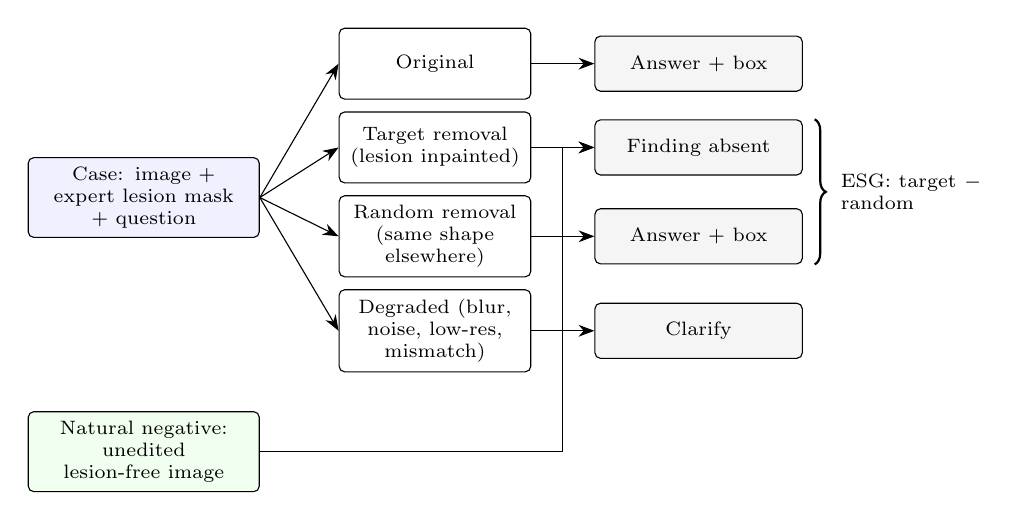
\begin{tikzpicture}[node distance=4mm and 6mm,
  box/.style={draw,rounded corners=2pt,align=center,font=\scriptsize,minimum height=9mm,text width=22mm},
  act/.style={draw,rounded corners=2pt,align=center,font=\scriptsize,fill=gray!8,text width=24mm,minimum height=7mm},
  >={Stealth[length=2mm]}]
\node[box,fill=blue!6,text width=27mm] (case) {Case: image $+$\\expert lesion mask\\$+$ question};
\node[box,right=10mm of case,yshift=17mm] (o) {Original};
\node[box,below=1.5mm of o] (t) {Target removal\\(lesion inpainted)};
\node[box,below=1.5mm of t] (r) {Random removal\\(same shape elsewhere)};
\node[box,below=1.5mm of r] (d) {Degraded (blur,\\noise, low-res,\\mismatch)};
\node[box,fill=green!6,text width=27mm,below=22mm of case] (n) {Natural negative:\\unedited\\lesion-free image};
\node[act,right=8mm of o] (ao) {Answer $+$ box};
\node[act,right=8mm of t] (at) {Finding absent};
\node[act,right=8mm of r] (ar) {Answer $+$ box};
\node[act,right=8mm of d] (ad) {Clarify};
\foreach \v in {o,t,r,d} \draw[->] (case.east) -- (\v.west);
\foreach \v/\a in {o/ao,t/at,r/ar,d/ad} \draw[->] (\v) -- (\a);
\draw[->] (n.east) -| ($(at.west)+(-4mm,0)$) -- (at.west);
\draw[decorate,decoration={brace,amplitude=4pt,mirror},thick] ($(ar.south east)+(1.5mm,0)$) -- node[right=2mm,font=\scriptsize,align=left] {ESG: target $-$\\random} ($(at.north east)+(1.5mm,0)$);
\end{tikzpicture}
\caption{Views built from each case and the expected action. Target removal and natural negatives share the expected reply and the reward; target and random removal share the editing operator and the edited shape, so only a model that reads the lesion can separate them (ESG).}
\label{fig:views}
\end{figure}

\subsection{Automated quality control}
No human checks any view. A case is kept only if (i) the lesion no longer stands out from its surroundings in the target-removal view, (ii) no lesion pixel changed in the random-removal view, and (iii) no view is a near-duplicate of a training image (perceptual hash, confirmed by pixel correlation). Splits are made over patients or groups of near-identical images; SLAKE's official split leaks neighbouring slices across splits (4 of 63 validation/test images had a near-copy in train), which group splitting removes. Finally, a texture classifier is trained to separate target-removal from random-removal edits; cases it separates most confidently are filtered until its AUC is at most 0.6 (Table~\ref{tab:data}). A learned ResNet-18 edit-trace detector is evaluated in Section~\ref{sec:edit}.

\subsection{Reward and net utility}
Each decision is scored with a clinical cost matrix (Table~\ref{tab:cost}), used both as the RL/selection reward and as the \emph{net utility} metric. A correct answer on an original view earns a grounding bonus of 0.5 when its box overlaps the lesion with IoU $\ge 0.3$ (boxes larger than half the image earn none). Unparseable output scores $-1$; tool calls beyond the first cost 0.05 each.

\begin{table}[t]
\centering\small
\caption{Cost matrix (reward per view). Target removal and natural negatives are identical by design.}
\label{tab:cost}
\setlength{\tabcolsep}{4pt}\begin{tabular}{lcccc}
\toprule
View & Correct / absent answer & Wrong or claims finding & Refer & Clarify \\
\midrule
Original, random removal & $+1.0$ & $-2.0$ ($-4.0$ critical) & $-0.3$ & $-0.3$ \\
Target removal & $+1.0$ & $-2.0$ & $+0.5$ & $-0.5$ \\
Natural negative & $+1.0$ & $-2.0$ & $+0.5$ & $-0.5$ \\
Degraded & $+0.25$ & $-2.0$ & $0.0$ & $+0.5$ \\
\bottomrule
\end{tabular}
\end{table}

\subsection{Training MedScope-4B}
The base model is Qwen3.5-4B with LoRA ($r=16$, $\alpha=32$, dropout 0.05, all linear layers of the language model; the vision encoder is frozen).

\paragraph{Stage 1: supervised fine-tuning on synthetic trajectories.} For every training view a multi-turn trajectory is generated from the labels alone: optionally a zoom on (a jittered box around) the lesion, then the expected final action with the lesion box, the absent answer, or a clarification request, with short template reasoning. 1 epoch over about 11,000 views (all five imaging types plus natural negatives), learning rate $2\times10^{-4}$, gradient accumulation 8, 1,980 optimiser steps.

\paragraph{Stage 2: rejection-sampling fine-tuning (RFT).} The stage-1 model samples 4 episodes on each of 150 training views per view kind; the highest-reward successful episode (correct answer, absent answer, or clarify on degraded input) is kept. At least one sample succeeded on 95--100\% of views. Training continues on the kept episodes plus 3,000 synthetic views (learning rate $5\times10^{-5}$, about 670 steps).

\paragraph{Stage 3: general-VQA replay (final model).} Because every stage-1/2 question concerns a lesion, the model learned to over-use ``No abnormality'' on open questions (``Where are the kidneys?''). We continue from RFT on 5,000 views that mix MedScope views with ordinary questions from the \emph{training} splits of VQA-RAD, SLAKE and PathVQA, excluding any image near-identical to an evaluation image (perceptual hash) and any SLAKE image in our validation or test sets (learning rate $5\times10^{-5}$). The rule for adopting the stage-3 model was fixed before testing: keep it if validation net utility is within 0.02 of RFT. It scored 0.804 against 0.801 and became the final model.

\paragraph{Explored and not used.} GRPO from the stage-1 agent, plain and with dynamic sampling, and seven adapter-merging schemes; Section~\ref{sec:negative}.

\subsection{Metrics}
Let $T$, $R$, $O$, $N$, $D$ denote target-removal, random-removal, original, natural-negative and degraded views.
\begin{itemize}[leftmargin=*,nosep]
\item \textbf{CCR} (covered-and-correct rate): fraction of answerable views ($O\cup R$) answered correctly.
\item \textbf{ESG} $= P(\text{absent answer or refer}\mid T) - P(\text{absent answer or refer}\mid R)$.
\item \textbf{Erased-lesion hallucination}: $P(\text{claims the finding}\mid T)$.
\item \textbf{Healthy-image hallucination}: $P(\text{claims the finding}\mid N)$.
\item \textbf{Grounded accuracy}: correct answer with IoU $\ge 0.3$ on $O$.
\item \textbf{Clarify rate} on $D$; \textbf{net utility}: mean reward over all views (Table~\ref{tab:cost}).
\item \textbf{AURC} with confidence equal to the geometric mean of the greedy probabilities of the answer tokens (stated confidence is also reported).
\end{itemize}
95\% confidence intervals use 2,000 bootstrap resamples of \emph{cases} (all views of a case move together). Model comparisons use a paired bootstrap on the cases both models were evaluated on, with two-sided $p$-values.

\subsection{Evaluation harness}\label{sec:harness}
All models are decoded greedily with the same prompt, the same tools and identical decoding settings (no repetition penalty or $n$-gram blocking from model-specific configs). Answers are parsed from the first action; answer matching accepts paraphrases and health-question polarity (``Is the liver healthy?'' $\to$ ``Healthy'' means yes) and reads the asked finding before other cues (``no pneumothorax'' is no; ``pneumothorax without mediastinal shift'' is yes). A reply with no action tag is read as the model's decision (a plain answer, or a request for a better image when it states the image is blurred, noisy, low resolution or the wrong image), identically for every model; the plain-prose rate is reported. Correctness and rewards are always recomputed from stored transcripts, so parsing rules are applied uniformly to every run. API models receive images as PNG with the long side at most 768 pixels and run with each provider's default reasoning settings.

\section{Experimental setup}

\subsection{Data}
Table~\ref{tab:data} lists the sources. Questions are generated from every image with a lesion mask (one question per image for the three added datasets) plus SLAKE's own abnormality questions. The main test set has 507 cases: 219 counterfactual cases with original, target-removal and random-removal views (170 also have a degraded view after mismatch views built without a different-modality guarantee were dropped) and 288 natural negatives; 1,115 views in total.

\begin{table}[t]
\centering\small
\caption{Training and evaluation data. Shortcut AUC: texture classifier separating target- from random-removal edits (before $\to$ after filtering).}
\label{tab:data}
\begin{tabular}{p{3.4cm}p{1.9cm}p{1.6cm}p{6.6cm}}
\toprule
Source & Imaging & Test cases & Notes \\
\midrule
Kvasir-SEG~\cite{kvasir} + HyperKvasir~\cite{hyperkvasir} & Colonoscopy & 174 & HyperKvasir normal landmarks (cecum, rectum, ileum) as negatives \\
SLAKE~\cite{slake} & CT / MRI & 107 & Group split; 179 masks with undocumented grey levels skipped \\
ChestX-Det~\cite{chestxdet} & Chest X-ray & 91 & Diffuse findings excluded (cardiomegaly, emphysema, diffuse nodules) \\
TCGA-LGG~\cite{lgg} & Brain MRI & 78 & Patient split; slices with little brain excluded \\
BUSI~\cite{busi} & Breast US & 57 & Lesions too large to erase excluded \\
\midrule
\multicolumn{4}{l}{Shortcut AUC, SLAKE/Kvasir: train 0.627$\to$0.594, val 0.628$\to$0.577, test 0.641$\to$0.562} \\
\multicolumn{4}{l}{Shortcut AUC, added datasets: train 0.602$\to$0.567, val 0.598, test 0.563} \\
\midrule
\multicolumn{4}{p{15cm}}{\textbf{External centres} (never used for training; 169 cases, 526 views):} \\
\multicolumn{4}{p{15cm}}{CVC-ClinicDB~\cite{cvc} (Barcelona), QaTa-COV19~\cite{qata} (Qatar), BUS-BRA~\cite{busbra} (Brazil), BraTS-Africa 2023~\cite{bratsafrica}} \\
\multicolumn{4}{p{15cm}}{\textbf{General VQA}: VQA-RAD test (451)~\cite{vqarad}, SLAKE English test (300 sampled)~\cite{slake}, PathVQA test (300 sampled)~\cite{pathvqa}} \\
\bottomrule
\end{tabular}
\end{table}

External sources were chosen so that no image is shared with a training source: SIIM pneumothorax and BraTS 2020/2021 were rejected because they overlap NIH ChestX-ray14 and TCGA. BraTS-Africa volumes are sliced at the axial FLAIR slice with the largest tumour, plus a tumour-free slice of the same patient at least 10 slices away.

\subsection{Models compared}
\textbf{Open models} (same harness, bf16, A100 40\,GB): Qwen3.5-4B (base of MedScope), MedGemma 1.5 4B~\cite{medgemma}, Qwen3-VL-8B, Qwen2.5-VL-7B~\cite{qwen25vl}, Lingshu-7B~\cite{lingshu}, HuatuoGPT-Vision-7B~\cite{huatuo}. \textbf{Frontier models} through their APIs with the identical agent loop: OpenAI gpt-6-sol, gpt-6-astra, gpt-6.1-sol; Anthropic Claude Fable 5.1, Opus 5.5, Sonnet 5.5; Google gemini-4-argon, gemini-3.1-pro-preview, gemini-3.8-flash. \textbf{Ablations}: the same SFT without counterfactual views (trained on original, natural-negative and degraded views only, same number of steps); the earlier refer-only agent; RFT without replay.

\section{Results}

\subsection{Main test}
Table~\ref{tab:main} gives the main results. MedScope-4B is as accurate as the best models on real lesions (CCR 0.881 vs 0.886--0.888 for gpt-6-astra and gpt-6.1-sol, $p>0.79$) but treats the erased lesion as absent far more often: it claims an erased lesion in 13.7\% of cases, against 49.8\% (gpt-6-sol) and 58.9\% (gpt-6-astra, gpt-6.1-sol). Its ESG of 0.744 is more than double that of any OpenAI model (0.306--0.347) and of every open baseline (at most 0.338). The difference also holds on \emph{unedited} healthy images (14.6\% vs 25.7--30.9\% false findings), which cannot be explained by editing artefacts.

\begin{table}[t]
\centering\small
\caption{Main test (507 cases, 1,115 views). Hallucination columns: claims the finding after the lesion was erased / on an unedited healthy image (lower is better). Net utility with 95\% bootstrap CI where available.}
\label{tab:main}
\footnotesize\setlength{\tabcolsep}{4pt}
\begin{tabular}{lcccccc}
\toprule
Model & CCR & ESG & Erased & Healthy & Grounded & Net utility \\
\midrule
\textbf{MedScope-4B (final, v3)} & 0.881 & \best{0.744} & 0.137 & 0.146 & \best{0.817} & \best{0.714} \\
MedScope-4B, RFT (no replay) & 0.865 & \best{0.758} & \best{0.114} & \best{0.083} & 0.813 & 0.752 [0.673, 0.829] \\
Refer-only agent (ablation) & 0.660 & 0.594 & 0.059 & 0.132 & 0.575 & 0.537 \\
\midrule
gpt-6-sol & 0.822 & 0.347 & 0.498 & 0.257 & 0.639 & 0.249 \\
gpt-6-astra & 0.886 & 0.306 & 0.589 & 0.278 & 0.717 & 0.309 \\
gpt-6.1-sol & \best{0.888} & 0.324 & 0.589 & 0.309 & 0.708 & 0.276 \\
Claude Fable 5.1 / Opus 5.5 / Sonnet 5.5 & \multicolumn{6}{c}{\pend{full runs in progress}} \\
gemini-4-argon / 3.1-pro / 3.8-flash & \multicolumn{6}{c}{\pend{full runs in progress}} \\
\midrule
Qwen3.5-4B (base) & 0.758 & 0.338 & 0.420 & 0.194 & 0.192 & 0.134 \\
Qwen3-VL-8B & 0.553 & 0.297 & 0.128 & 0.125 & 0.388 & 0.186 \\
MedGemma 1.5 4B & 0.660 & 0.169 & 0.534 & 0.240 & 0.137 & $-0.417$ \\
Qwen2.5-VL-7B\dag & 0.144 & $-0.059$ & 0.055 & 0.247 & 0.005 & $-0.946$ \\
Lingshu-7B\dag & 0.005 & 0.000 & 0.000 & 0.000 & 0.000 & $-0.953$ \\
HuatuoGPT-Vision-7B\dag & 0.000 & 0.000 & 0.000 & 0.000 & 0.000 & $-1.000$ \\
\bottomrule
\multicolumn{7}{p{14cm}}{\footnotesize \dag{} Answers mostly in plain prose (Lingshu 96\%, HuatuoGPT 100\%, Qwen2.5-VL 35\%); \pend{rescored values from notebook 13}.}
\end{tabular}
\end{table}

\begin{table}[t]
\centering\small
\caption{MedScope-4B (final) vs frontier models, paired bootstrap over the same 507 cases (difference = MedScope $-$ other).}
\label{tab:frontier}
\begin{tabular}{llccc}
\toprule
Compared with & Metric & MedScope & Other & Difference [95\% CI], $p$ \\
\midrule
\multirow{4}{*}{gpt-6-sol} & ESG & 0.744 & 0.347 & $+0.397$ [$+0.313$, $+0.475$], $<$0.001 \\
 & Erased-lesion claims & 0.137 & 0.498 & $-0.361$ [$-0.434$, $-0.285$], $<$0.001 \\
 & Healthy-image claims & 0.146 & 0.257 & $-0.111$ [$-0.173$, $-0.050$], 0.001 \\
 & Net utility & 0.714 & 0.249 & $+0.466$ [$+0.378$, $+0.557$], $<$0.001 \\
\midrule
\multirow{4}{*}{gpt-6-astra} & ESG & 0.744 & 0.306 & $+0.438$ [$+0.356$, $+0.520$], $<$0.001 \\
 & Erased-lesion claims & 0.137 & 0.589 & $-0.452$ [$-0.523$, $-0.380$], $<$0.001 \\
 & Healthy-image claims & 0.146 & 0.278 & $-0.132$ [$-0.197$, $-0.073$], $<$0.001 \\
 & Net utility & 0.714 & 0.309 & $+0.406$ [$+0.317$, $+0.501$], $<$0.001 \\
\midrule
\multirow{4}{*}{gpt-6.1-sol} & ESG & 0.744 & 0.324 & $+0.420$ [$+0.342$, $+0.503$], $<$0.001 \\
 & Erased-lesion claims & 0.137 & 0.589 & $-0.452$ [$-0.528$, $-0.380$], $<$0.001 \\
 & Healthy-image claims & 0.146 & 0.309 & $-0.163$ [$-0.232$, $-0.099$], $<$0.001 \\
 & Net utility & 0.714 & 0.276 & $+0.438$ [$+0.350$, $+0.535$], $<$0.001 \\
\midrule
\multicolumn{5}{l}{CCR: $+0.059$ vs gpt-6-sol ($p=0.004$); $-0.005$ vs gpt-6-astra ($p=0.91$); $-0.007$ vs gpt-6.1-sol ($p=0.80$).} \\
\multicolumn{5}{l}{\pend{Claude and Gemini rows; paired tests vs all open baselines from notebook 13}} \\
\bottomrule
\end{tabular}
\end{table}

A typical frontier failure on an erased polyp is a confident description with a box where the polyp used to be (``a large sessile polyp occupying the central portion''). In 20-case pilot runs of the other six frontier models, erased-lesion claims ranged from 33\% (Claude Fable 5.1, Sonnet 5.5) to 50\% (Claude Opus 5.5, gemini-4-argon) on 12 erased-lesion views each; the full runs will replace these figures.

\subsection{What produces the behaviour: ablation}
Table~\ref{tab:ablation} compares stage-1 SFT with the identical recipe minus the counterfactual (target- and random-removal) views, trained for the same number of steps. Without counterfactual views the model answers ``Yes'' more readily, which slightly helps on real lesions (CCR $+0.053$) but more than quadruples erased-lesion claims (11.9\% $\to$ 53.0\%) and more than doubles false findings on unedited healthy images (8.7\% $\to$ 22.2\%), even though natural negatives were in its training data. The effect is the same at external centres. Per imaging type (Table~\ref{tab:types}), the ablation's erased-lesion claims reach 82\% on SLAKE CT/MRI and 73\% on chest X-ray.

\begin{table}[t]
\centering\small
\caption{Ablation: SFT with vs without counterfactual views (paired bootstrap). Main test 507 cases; external 169 cases.}
\label{tab:ablation}
\begin{tabular}{lccccc}
\toprule
 & \multicolumn{2}{c}{Main test} & \multicolumn{2}{c}{External centres} \\
\cmidrule(lr){2-3}\cmidrule(lr){4-5}
Metric & With CF & Without CF & With CF & Without CF \\
\midrule
ESG & \best{0.758} & 0.402$^{***}$ & \best{0.655} & 0.479$^{**}$ \\
Erased-lesion claims & \best{0.119} & 0.530$^{***}$ & \best{0.109} & 0.412$^{***}$ \\
Healthy-image claims & \best{0.087} & 0.222$^{***}$ & \best{0.080} & 0.360$^{***}$ \\
CCR & 0.877 & \best{0.929}$^{***}$ & 0.761 & \best{0.895}$^{***}$ \\
Net utility & \best{0.760} & 0.494$^{***}$ & \best{0.519} & 0.436 ($p=0.19$) \\
\bottomrule
\multicolumn{5}{l}{\footnotesize $^{**}p\le0.001$, $^{***}p<0.001$, paired bootstrap over cases.}
\end{tabular}
\end{table}

\begin{table}[t]
\centering\small
\caption{By imaging type, main test: MedScope-4B (RFT) and the no-counterfactual ablation. \pend{final model (v3) rows from notebook 13}.}
\label{tab:types}
\begin{tabular}{llcccccc}
\toprule
Model & Imaging & Cases & CCR & ESG & Erased & Healthy & Net \\
\midrule
\multirow{5}{*}{MedScope (RFT)} & Colonoscopy & 174 & 0.95 & 0.94 & 0.01 & 0.00 & 1.03 \\
 & Brain MRI & 78 & 0.92 & 0.83 & 0.08 & 0.02 & 0.87 \\
 & Breast US & 57 & 0.93 & 0.71 & 0.21 & 0.13 & 0.82 \\
 & SLAKE CT/MRI & 107 & 0.56 & 0.59 & 0.00 & 0.17 & 0.24 \\
 & Chest X-ray & 91 & 0.72 & 0.44 & 0.29 & 0.12 & 0.41 \\
\midrule
\multirow{5}{*}{Without CF} & Colonoscopy & 174 & 0.99 & 0.42 & 0.57 & 0.00 & 0.75 \\
 & Brain MRI & 78 & 0.90 & 0.67 & 0.22 & 0.02 & 0.74 \\
 & Breast US & 57 & 0.90 & 0.50 & 0.40 & 0.20 & 0.62 \\
 & SLAKE CT/MRI & 107 & 0.82 & 0.06 & 0.82 & 0.58 & $-0.46$ \\
 & Chest X-ray & 91 & 0.90 & 0.17 & 0.73 & 0.16 & 0.37 \\
\bottomrule
\end{tabular}
\end{table}

\subsection{External centres}
On 169 cases from four centres not used in training, the final model reaches CCR 0.773, ESG 0.672, erased-lesion claims 10.1\%, healthy-image claims 10.0\% and net utility 0.522 (RFT: ESG 0.664, net 0.534 [0.414, 0.650]; no significant difference between the two). Open baselines reach ESG 0.328 (Qwen3.5-4B), 0.227 (Qwen3-VL-8B) and 0.185 (MedGemma 1.5), all $p<0.001$ against MedScope. By source (RFT), ESG is 0.93 on BraTS-Africa, 0.80 on CVC-ClinicDB, 0.69 on BUS-BRA and 0.15 on QaTa-COV19, where diffuse COVID-19 opacities are erased far less completely than focal lesions (45\% erased-opacity claims). \pend{frontier models on external centres: not run; decide whether needed}.

\subsection{General medical VQA}
Table~\ref{tab:vqa} shows that the final model does not trade general ability for evidence sensitivity. Before replay (RFT), open-question accuracy collapsed (SLAKE open 0.215) because the model answered ``No abnormality'' to anatomical questions; replay restores and exceeds the base model on all three benchmarks. The final model was trained on the training splits of these benchmarks (evaluation images excluded) while the base model is zero-shot, so these numbers show the absence of a regression rather than a like-for-like comparison with zero-shot models.

\begin{table}[t]
\centering\small
\caption{Standard medical VQA accuracy (closed / open / all), same agent prompt and answer matching for every model.}
\label{tab:vqa}
\begin{tabular}{lccc}
\toprule
Model & VQA-RAD (451) & SLAKE test (300) & PathVQA (300) \\
\midrule
MedScope-4B (final) & \best{0.777} / \best{0.275} / \best{0.554} & \best{0.899} / \best{0.691} / \best{0.767} & \best{0.833} / \best{0.181} / \best{0.520} \\
MedScope-4B (RFT, no replay) & 0.673 / 0.090 / 0.415 & 0.688 / 0.215 / 0.387 & 0.500 / 0.000 / 0.260 \\
Qwen3.5-4B (base, zero-shot) & 0.657 / 0.260 / 0.481 & 0.826 / 0.424 / 0.570 & 0.545 / 0.021 / 0.293 \\
MedGemma 1.5 4B (all) & 0.379 & 0.407 & 0.230 \\
Qwen3-VL-8B (all) & 0.452 & 0.477 & 0.250 \\
\bottomrule
\end{tabular}
\end{table}

\subsection{Is the model detecting edits?}\label{sec:edit}
Three results argue against an edit-detection explanation. (i) By construction, an edit detector scores ESG $=0$, since both target- and random-removal views are edited; MedScope denies or refers on only a small fraction of random-removal views while doing so on most target-removal views. (ii) The hallucination reduction holds on \emph{unedited} lesion-free images (Tables~\ref{tab:main} and \ref{tab:ablation}). (iii) The adversarially filtered shortcut AUC on test is 0.56. \pend{learned ResNet-18 edit-trace detector, random removal vs original (both show the lesion, one edited): AUC from notebook 13}.

\subsection{Calibration}
Fine-tuning collapsed the stated confidence to nearly a constant ($\approx$0.81; AURC 0.171 for RFT), but the probability of the answer tokens ranks right and wrong answers well (AURC 0.022 on test, 0.053 at external centres). \pend{final-model AURC}.

\subsection{What did not help}\label{sec:negative}
\paragraph{On-policy RL.} Plain GRPO from the stage-1 agent (150 steps, 4 episodes per image) left the model unchanged: only 20\% of sampled groups had any reward difference, so group-relative advantages vanished. Dynamic sampling (8 episodes per image, images drawn until 2 groups had signal) gained one validation case (net utility 0.844 $\to$ 0.878, overlapping CIs) as the policy grew more deterministic. Rejection sampling, which learns from any single success among samples, was more productive and is used instead.
\paragraph{Adapter merging.} Merging a grounding-only adapter into the agent (linear SVD, concatenation, TIES, DARE-TIES) never beat the agent alone; net utility fell from 0.891 to 0.21 as grounding weight increased, and the abstention gap fell from 0.900 to 0.000 while grounded accuracy stayed at 0.85--0.93. Merging keeps perception and removes evidence sensitivity.
\paragraph{Grounding supervision alone.} An adapter trained only to answer with boxes reached 0.90 grounded accuracy but claimed the finding on 100\% of erased and of naturally lesion-free images.

\section{Discussion}
The central result is that the ability to \emph{see} a lesion and the disposition to \emph{report only what is seen} are separable. Frontier models detect lesions as well as MedScope-4B but report them about half the time after they are gone; a 4B model acquires the disposition from automatically built counterfactuals and nothing else, and the ablation identifies those counterfactuals as the active ingredient. Because the views come from public masks and the checks are automatic, the recipe extends to any dataset with segmentation labels.

The final model trades a small amount of healthy-image specificity for general question answering (healthy-image false findings 8.3\% $\to$ 14.6\% with replay, $p<0.001$; ESG unchanged). Practitioners can choose either checkpoint; both are released.

\paragraph{Limitations.}
\begin{itemize}[leftmargin=*,nosep]
\item \textbf{No clinician review.} The views are checked automatically, and evaluation uses dataset labels only. Realism of the inpainted images is argued through the matched control, unedited negatives and edit-trace detection, not human reading.
\item \textbf{Diffuse findings.} Erasing diffuse opacities is incomplete (QaTa-COV19 ESG 0.15); the method suits focal lesions.
\item \textbf{2D only.} CT and MRI are evaluated as single slices.
\item \textbf{Label noise.} Some SLAKE ``healthy'' labels may be wrong; this affects every model equally. \pend{manual check of a sample}.
\item \textbf{Single training seed} and a single base model. \pend{additional seeds if compute allows}.
\item \textbf{Frontier models} are evaluated with their default settings and our prompt; prompt variants are not explored. \pend{cautious-prompt sensitivity check}.
\end{itemize}

\section{Conclusion}
Counterfactual lesion erasure with an edit-matched control turns ``does the model report what the image shows?'' into a measurable and trainable property. Trained on such views without any human annotation, a 4B agent matches frontier models on real lesions and hallucinates erased findings three to four times less often, at its training sites and at four external centres, while keeping general medical VQA ability.

\paragraph{Data and code availability.} Code, view-building recipes, the benchmark and model weights: \url{https://github.com/bhaskargurram-ai/medscope} \pend{Hugging Face links}. MedScope is a research model and not a medical device.

\begin{thebibliography}{99}\small
\bibitem{llavamed} C.~Li et al. LLaVA-Med: Training a large language-and-vision assistant for biomedicine in one day. \emph{NeurIPS Datasets and Benchmarks}, 2023.
\bibitem{huatuo} J.~Chen et al. HuatuoGPT-Vision: Towards injecting medical visual knowledge into multimodal LLMs at scale. \emph{EMNLP}, 2024.
\bibitem{medgemma} A.~Sellergren et al. MedGemma technical report. arXiv, 2025.
\bibitem{lingshu} LASA Team (Alibaba DAMO). Lingshu: A generalist foundation model for unified multimodal medical understanding and reasoning. arXiv, 2025.
\bibitem{qwen25vl} S.~Bai et al. Qwen2.5-VL technical report. arXiv, 2025.
\bibitem{vqarad} J.~J.~Lau et al. A dataset of clinically generated visual questions and answers about radiology images. \emph{Scientific Data}, 2018.
\bibitem{slake} B.~Liu et al. SLAKE: A semantically-labeled knowledge-enhanced dataset for medical visual question answering. \emph{ISBI}, 2021.
\bibitem{pathvqa} X.~He et al. PathVQA: 30000+ questions for medical visual question answering. arXiv, 2020.
\bibitem{pope} Y.~Li et al. Evaluating object hallucination in large vision-language models. \emph{EMNLP}, 2023.
\bibitem{cares} P.~Xia et al. CARES: A comprehensive benchmark of trustworthiness in medical vision language models. \emph{NeurIPS}, 2024.
\bibitem{medhallmark} J.~Chen et al. Detecting and evaluating medical hallucinations in large vision language models (Med-HallMark). arXiv, 2024.
\bibitem{medvh} Z.~Gu et al. MedVH: Towards systematic evaluation of hallucination for large vision language models in the medical context. arXiv, 2024.
\bibitem{lama} R.~Suvorov et al. Resolution-robust large mask inpainting with Fourier convolutions. \emph{WACV}, 2022.
\bibitem{aurc} Y.~Geifman and R.~El-Yaniv. Selective classification for deep neural networks. \emph{NeurIPS}, 2017.
\bibitem{star} E.~Zelikman et al. STaR: Bootstrapping reasoning with reasoning. \emph{NeurIPS}, 2022.
\bibitem{rft} Z.~Yuan et al. Scaling relationship on learning mathematical reasoning with large language models. arXiv, 2023.
\bibitem{grpo} Z.~Shao et al. DeepSeekMath: Pushing the limits of mathematical reasoning in open language models. arXiv, 2024.
\bibitem{dapo} Q.~Yu et al. DAPO: An open-source LLM reinforcement learning system at scale. arXiv, 2025.
\bibitem{lora} E.~J.~Hu et al. LoRA: Low-rank adaptation of large language models. \emph{ICLR}, 2022.
\bibitem{kvasir} D.~Jha et al. Kvasir-SEG: A segmented polyp dataset. \emph{MMM}, 2020.
\bibitem{hyperkvasir} H.~Borgli et al. HyperKvasir, a comprehensive multi-class image and video dataset for gastrointestinal endoscopy. \emph{Scientific Data}, 2020.
\bibitem{chestxdet} J.~Lian et al. A structure-aware relation network for thoracic diseases detection and segmentation (ChestX-Det). \emph{IEEE TMI}, 2021.
\bibitem{lgg} M.~Buda, A.~Saha, M.~A.~Mazurowski. Association of genomic subtypes of lower-grade gliomas with shape features automatically extracted by a deep learning algorithm. \emph{Computers in Biology and Medicine}, 2019.
\bibitem{busi} W.~Al-Dhabyani et al. Dataset of breast ultrasound images. \emph{Data in Brief}, 2020.
\bibitem{cvc} J.~Bernal et al. WM-DOVA maps for accurate polyp highlighting in colonoscopy (CVC-ClinicDB). \emph{Computerized Medical Imaging and Graphics}, 2015.
\bibitem{qata} A.~Degerli et al. OSegNet / QaTa-COV19: COVID-19 infection map generation and detection from chest X-ray images. \emph{Health Information Science and Systems}, 2021.
\bibitem{busbra} W.~G\'omez-Flores et al. BUS-BRA: A breast ultrasound dataset for assessing computer-aided diagnosis systems. \emph{Medical Physics}, 2024.
\bibitem{bratsafrica} M.~Adewole et al. The Brain Tumor Segmentation (BraTS) Challenge 2023: Glioma segmentation in sub-Saharan Africa patient population (BraTS-Africa). arXiv, 2023.
\end{thebibliography}

\appendix
\section{System prompt (identical for every model)}\label{app:prompt}
\begin{lstlisting}
You are MedScope, a careful medical imaging assistant used for research. You look at a medical image and answer a question about it from what the image actually shows: you report a finding only when you can see it, and you say so when it is not there.

On each turn, think briefly in plain text, then write exactly ONE action as a tagged JSON object and stop. After a tool call, stop and wait: you will be shown the result before you continue.

Example of a tool turn:
The lesion may be small, so I will look closer at the upper left. <tool>{"name": "zoom", "box": [100, 150, 450, 500]}</tool>
Example of a final turn:
The mass is clearly visible. <final>{"action": "answer", "answer": "Yes", "box": [180, 220, 320, 360], "confidence": 0.85}</final>

Tools (at most 3 calls per case; boxes are integers 0-1000 on the ORIGINAL full image, as [x1, y1, x2, y2]):
<tool>{"name": "zoom", "box": [x1, y1, x2, y2]}</tool>   look closer at a region
<tool>{"name": "window", "center": 128, "width": 100}</tool>   adjust brightness/contrast (0-255 scale)

Final actions (exactly one, then stop):
<final>{"action": "answer", "answer": "...", "box": [x1, y1, x2, y2], "confidence": 0.0-1.0}</final>
    when the image lets you answer. If the finding is visible, the box marks it on the original image.
    If the finding asked about is not there, say so and leave out the box: "No" to "Is there ...?",
    "Yes" to "Is ... healthy?" or "Is ... normal?", "No abnormality" to an open question.
<final>{"action": "clarify", "question": "..."}</final>
    when the image is unusable (too blurred, noisy, low resolution, or not the anatomy asked about).
<final>{"action": "refer", "reason": "..."}</final>
    when the image is usable but you cannot decide either way.

Keep answers short, using the wording a radiologist would use (for example "Yes", "No", "Liver", "Left lung"). Never report a finding you cannot see.
\end{lstlisting}

\section{Reproducibility}
Every stage runs on a single A100 40\,GB in Google Colab: stage-1 SFT about 4 hours, RFT about 4 hours, replay about 4 hours, full evaluation of one local model on the main test about 1 hour. Frontier evaluation runs on CPU; measured API cost for all nine models on the full test set is reported in the repository \pend{final cost table}. All evaluation results are stored as per-view transcripts and rescored by a single script, so every number in this paper can be regenerated from the released transcripts.

\end{document}
